\documentclass[../main.tex]{subfiles}	



\begin{document}
	
\chapter{Complex-Valued vs Real Neural Networks}

\section*{Introduction and Chapter Organization}

\section{Impact of the Circularity}

In chapter \ref{sec:circularity} we dedicated a whole section to the discussion about the circularity property of a complex random variable: we provided rigorous definitions of the circularity and the correlation coefficients, together with a brief explanation of their geometrical interpretation. We also cited a recent work by Barracchina et al. \cite{barrachina2021complexvalued}, suggesting the impact that datasets with such properties could have in machine learning applications. The authors, in fact, set up a classification task with two different distributions at a given circularity value, and then they use these to train real and complex-valued models. However they focused mostly on the training stability rather then on the difference in term of performances, that we, instead, believe could bring to very interesting results. For this reason, we decided to set up a similar problem in order to confirm first what they obtained, and then to come up with a more quantitative analysis of the accuracy that complex models can effectively achieve.

\subsection*{Data Generation}

The idea behind this analysis is to understand how much complex-valued models can effectively benefit of data with good circularity properties. For this reason we will generate two distinct complex-valued datasets, one with high correlations among real and imaginary components, and one with poor correlations.\\
An easy way to generate data with pre-determined circularity is to rely on the \textit{complex normal distribution}, that characterizes complex random variables whose real and imaginary parts are jointly normal. So, we can construct the samples we need simply exploiting the \texttt{multivariate random normal} distribution, supported by \texttt{numpy}: we just need to generate two-dimensional values that will constitute the real and imaginary parts of our data. Recalling the definition of the circularity coefficient
\[ \rho_z = \frac{\sigma_x^2 - \sigma_y^2}{\sigma_x^2 + \sigma_y^2} + i\frac{2\sigma_{xy}}{\sigma_x^2 + \sigma_y^2} \]
we can then tune the covariance matrix $\Gamma$ of the generating distribution to regulate the two main sources of non-circularity:
\[ \Gamma=\mqty(\sigma_x^2 & \sigma_{xy} \\ \sigma_{xy} & \sigma_y^2) \qquad\qquad  (I)\quad\sigma_x\neq\sigma_y \qquad\qquad (II)\quad\sigma_{xy}\neq 0 \]

As in the paper discussed above, we want to setup a classification problem among data following two different distributions:
\begin{itemize}
	\item with label "0", a perfectly circular complex normal ($\rho_z=0$), with zero-centered data and the identity as covariance matrix;
	\item with label "1", still a complex normal with mean zero, but with an arbitrary covariance matrix (variable $\rho_z$).
\end{itemize}
In practice, we will construct a dataset made of 5000 samples for each distribution, with each of them being constituted by 128 complex values. In figure \ref{fig:circ_class_example} we represent an example for each class of data. Successively the dataset will be partitioned in a train and a test set with proportions $80\%-20\%$.\\
\begin{figure}[!ht]
	\centering
	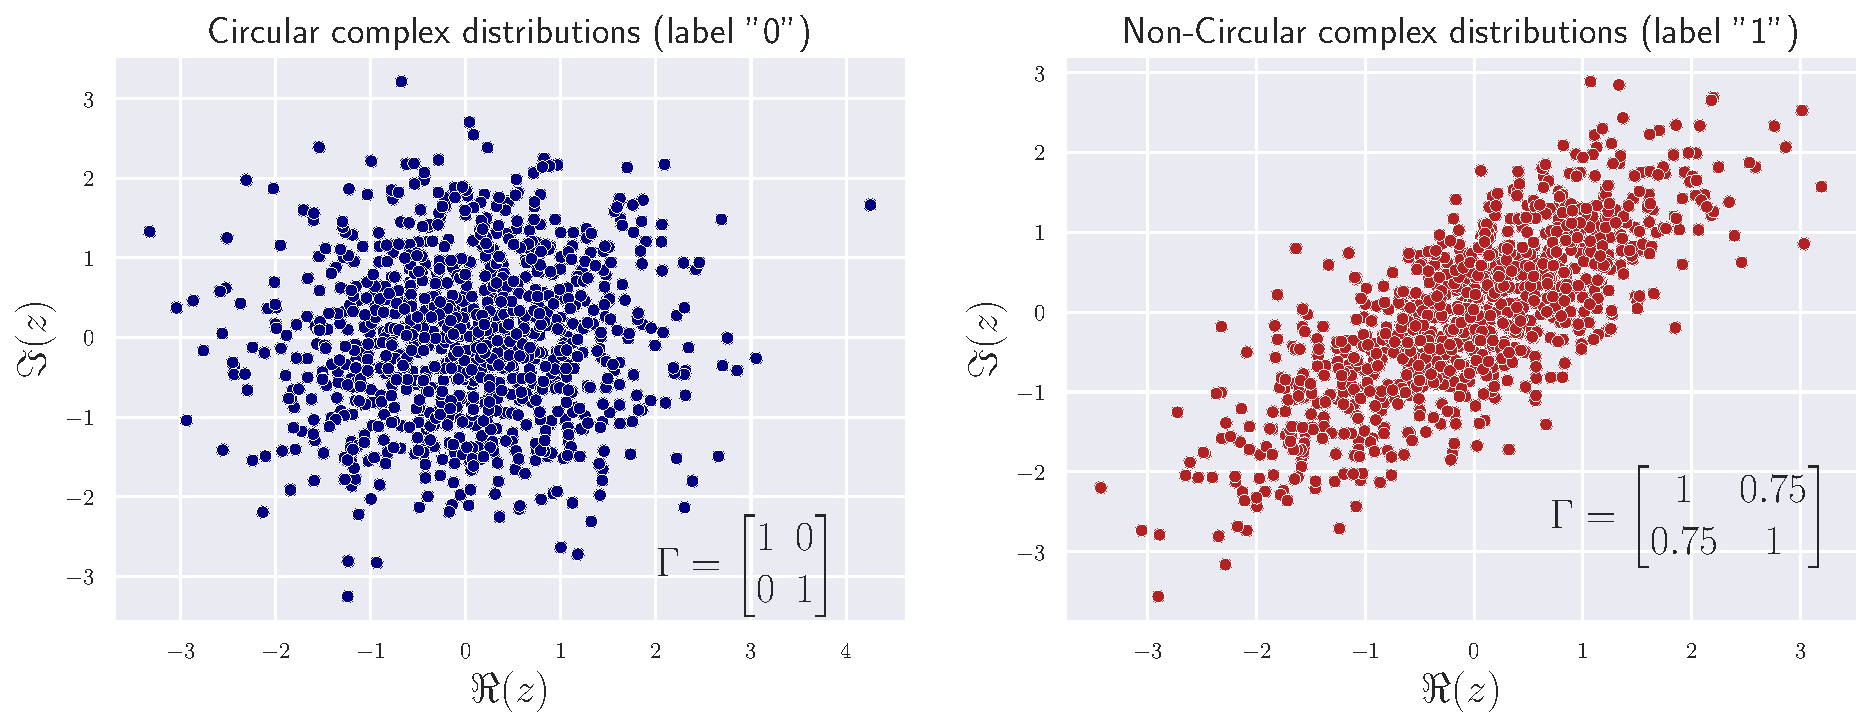
\includegraphics[width=\textwidth]{pictures/circ_class_example}
	\caption{Samples coming from a perfectly circular distribution (left) and from a non-circular one (right).}
	\label{fig:circ_class_example}
\end{figure}
It is important to note that the distinction between the classes is entirely contained in the relationship between the real and imaginary parts. This means that removing, for example, the imaginary part of the dataset will result in both classes being statistically identical, and therefore, making the classification impossible.

\subsection*{Classification Task}

To complete our setup, we just need to define a couple of neural networks to train: a complex-valued model, and its equivalent real-valued counterpart (treating the real and imaginary parts of the input as two independent channels) with double parameters respect to the first one. Datasets are quite simple by themselves, and so we used very elementary classifiers: we used a complex network with a couple of hidden layers (64 and 16 units respectively), and a small dropout ($20\%$). The same structure has been duplicated over two independent channels to obtain the real-valued network.\\
We made our tests for different label 1 distributions (changing the second covariance matrix while leaving the first equal to the identity), seeing that both models are able to learn easily from the dataset reaching also high accuracies ($>95\%$). But we also noticed that there are some configurations for which one of them outperform the other, sometimes even by a lot. In order to better investigate this situation, we proceed examining the two sources of non-circularity separately. Just to remark, the samples labeled with "0" have:
\[ \sigma_x = \sigma_y = 1 \qquad \sigma_{xy}=0 \qquad \implies \rho_z= \rho = 0 \]
Let's examine the first source of non-circularity in a complex distribution, i.e. data with a non-zero covariance factor ($\sigma_{xy}=0$). Considering the distribution "1", let's fix, for simplicity, $\sigma_x=\sigma_y=\sigma=1$ and leave the covariance $\sigma_{xy}$ free to space the interval $(-1,1)$ (to keep the covariance matrix positive defined). In this case we will have: $\rho_z=i\sigma_{xy}/\sigma^2$, $\rho=\sigma_{xy}/\sigma^2$ and so $\abs{\rho_z}=\abs{\rho}$.\\
We generated several datasets with the setup just described (fixed variances but different $\sigma_{xy}$) and trained both models over all of them for 60 epochs. As final "performance score" we kept the average classification computed over the last 10 epochs for the test set. To improve the reliability of the statistics found, we repeated the entire procedure for different random seeds (taken into account in the errorbars of the plots) and represented the results in figure \ref{fig:noncirc_results} (left). The behavior of the points is quite clear and regular: for this kind of non-circularity, the complex model outperforms the real one, also by a significative percentage, as the modulus of the circularity coefficient $\rho_z$ approaches 1 (and so does the correlation $\rho$).\\
Then we examined also the second source of non-circularity, i.e. different variances among real and imaginary parts of the variables $(\sigma_x\neq\sigma_y)$. This time we started fixing $\sigma_{xy}=0$ and also, for simplicity, $\sigma_x=1$ (because, in the end, it is just the shape of the distribution that matters). We leaved, instead, the second variance $\sigma_y$ free to move in an interval $(0, 3]$. This time we have $\rho_z= (\sigma_x^2-\sigma_y^2)/ (\sigma_x^2+\sigma_y^2)$ and $\rho=0$.\\
We repeated again the same procedure as for the first source and obtained the results in figure \ref{fig:noncirc_results} (right). The behavior of the accuracies is again quite clear and regular, but this time we see the real model performing better than its complex-valued counterpart; however, this advantage is relatively small, and seems to completely vanish as $\abs{\rho_z}$ approaches 1. A possible justification to this behavior stands on the fact that the real and imaginary part of the data are statistically not correlated, since $\rho=0$. We believe, in fact, that the two independent channels of the real model are probably more adapt to learn such internal structure with respect to the complex-valued architecture, whose parameters still preserve some local correlations, even after the training loop.\\
\begin{figure}[!ht]
	\centering
	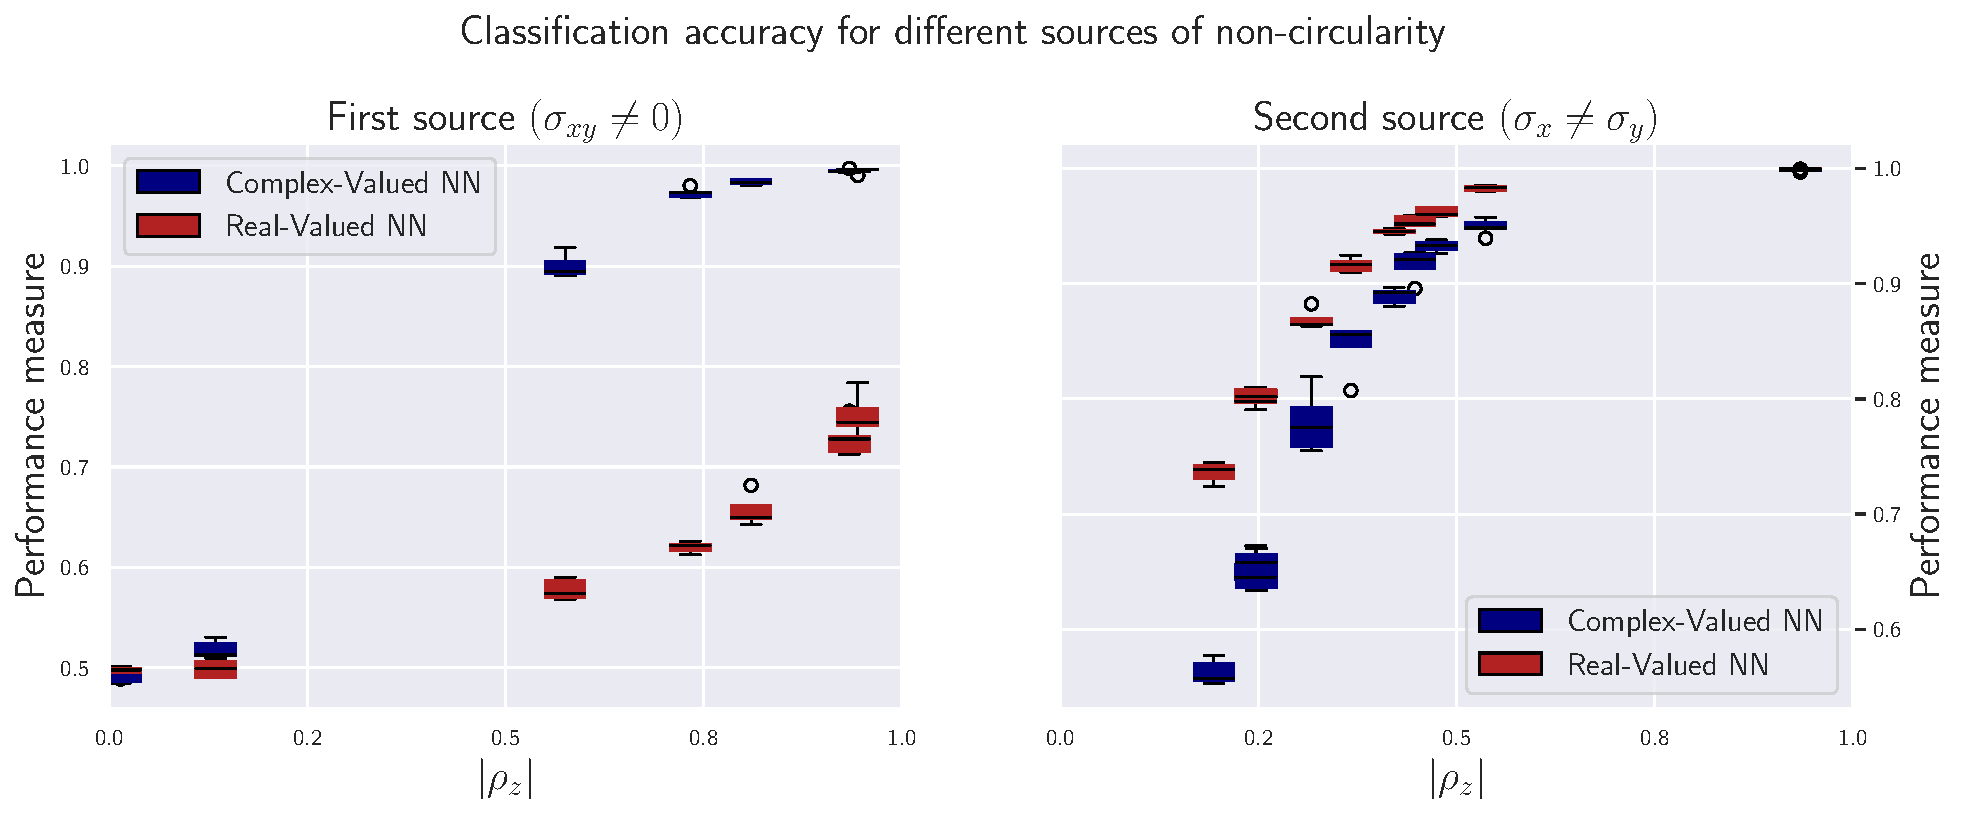
\includegraphics[width=\textwidth]{pictures/noncirc_results}
	\caption{Classification accuracy for real and complex-valued networks as function of different source of non-circularity.}
	\label{fig:noncirc_results}
\end{figure}
In the previous analysis we found some really interesting regular behaviors, with situations in which complex models are dominating and others in which are the real ones performing better. But, is there any general law, or rule, that we can find, in order to understand which characteristics should our data have, in order to guarantee nice performances for complex networks?\\
Let's proceed in the same way as before, fixing a distribution "0" that is perfectly circular, again with the identity as covariance matrix, and let's try to distinguish its samples from the ones coming from a second distribution "1", in which we add some non-circularity from both sources. We decide again to fix $\sigma_x=1$ for the second distribution, while the two remaining degrees of freedom $\sigma_y$ and $\sigma_{xy}$ are let free. Let's vary those parameter in order to space all the possible values that $\rho_z$ can assume, i.e. all the points in the unitary complex circle, and train again the models.\\
Because of the finite precision and the low amount of points in our samples (128), we cannot construct an accurate and uniform grid spacing all the possible values, and so we decided to adopt a stochastic method: sampling random combinations of $(\sigma_y, \sigma_{xy})$, computing the relative performance measure for the architectures, and reconstructing the accuracy distribution with the functionality \texttt{tri.LinearTriInterpolator}, provided by \texttt{matplotlib}. The final results of this analysis are presented in figure \ref{fig:noncirc_comparison_final}
\begin{figure}[!ht]
	\centering
	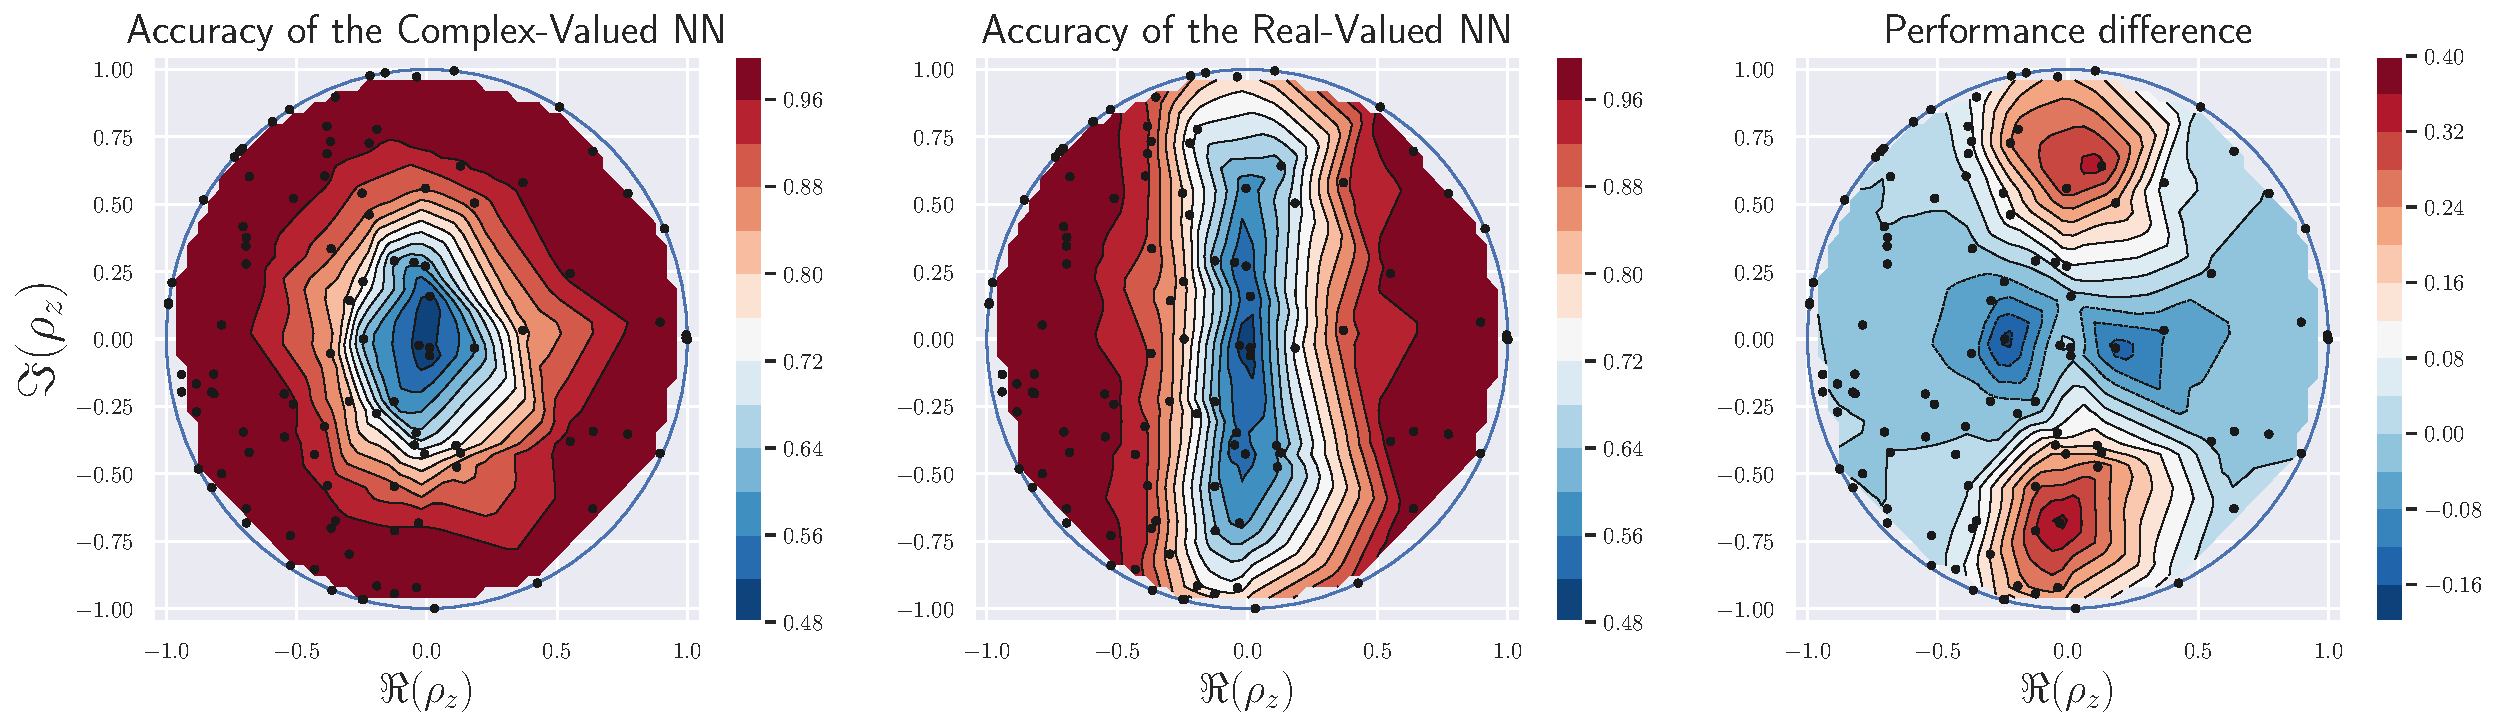
\includegraphics[width=\textwidth]{pictures/noncirc_comparison_final}
	\caption{Comparison of the accuracy achieved by a complex-valued model (left) and its real equivalent counterpart (center) in distinguishing a perfectly circular distribution from a second one as function of its circularity quotient.}
	\label{fig:noncirc_comparison_final}
\end{figure}




\section{Complex vs Real Models}
	
	
	
\end{document}